\chapter{Adaptive Learning}
\label{chap:adaptive-learning}

% TODO:
% - incorporate other notes from my/thesis gdoc
% - inspiration from relevant articles
% - add references for provided examples (playing chess, autonomous car, ...)

From playing chess to driving an autonomous car,
  artificial intelligence proved to be a mighty tool
  for tackling difficult algorithmic tasks.
The power of artificial intelligence can be also used
  to develop a personalized adaptive system for learning programming.
Such system would create an optimal learning experience for each student
  by providing them with problems of difficulty matching their skill,
  so that the student stays challenged and interested in solving them.

TODO: terminology note: Intelligent tutoring systems (ITS)
  (REF e.g. Hyacinth S. Nwana. Intelligent tutoring systems: an overview)
  (? is ITS = adaptive learning system, or is AL too specific term - just
  one of more possible strategies?)

In the existing systems (\ref{sec:existing-systems}),
  the sequence of tasks is the same for everybody.
As a result, the progress is necessarily too slow for some students,
  who could skip some of the tasks,
  while being too fast for others,
  who could highly benefit from solving a couple of other similar tasks.
Artificial intelligence can be used to personalize
  the sequence of tasks for every student.
By giving the student a suitable task
  -- neither too easy, nor too difficult --
  it can help the student to get into the state of flow
  (\ref{sec:motivation.challenge}).

In addition to choosing the most suitable task for given student,
  artificial intelligence has also other possible uses in learning systems,
  for example automatic hints generation \cite{generating-hints},
  cheating detection (REF),
  or skills visualization (REF).
Furthermore, artificial intelligence techniques can be used
  to analyze collected data offline.
Such analyses can reveal problematic tasks,
  or suggest how to group tasks into problem sets (TBA: ref).

Adaptive learning systems have been already successful in some domains.
For instance, Map Outlines%
  \footnote{Available at \url{https://outlinemaps.org}.},
  developed by Adaptive Learning research group at Masaryk University,
  is an intelligent web application for learning geography.
It has been used by tens of thousands of students
  and online experiments have confirmed
  that the adaptivity of the system helps to improve the learning outcome
  \cite{alg.evaluation-geography}.
In addition to geography, similar adaptive web applications
  for learning anatomy%
  \footnote{Available at \url{https://practiceanatomy.com}.},
  biology%
  \footnote{Available at \url{https://poznavackaprirody.cz} (in Czech only).},
  elementary mathematics%
  \footnote{Available at \url{https://matmat.cz} (in Czech only).},
  and Czech grammar%
  \footnote{Available at \url{https://umimecesky.cz} (in Czech only).},
  were developed by the research group in recent years.

TODO:
- mention other famous ITS (Duolingo);
- specifically name ITS' related to programming - refs to the previous
chapter (Umime programovat, Tutor)


Sections \ref{sec:domain-modeling} and \ref{sec:student-modeling} present how
to model the domain and students of the introductory programming.
Sections \ref{sec:task-recommendation} and \ref{sec:mastery-learning}
then describe two different uses of these models to make a learning system
personalized, namely adaptive task recommendation, and mastery learning.
Finally, section \ref{sec:metrics-and-evaluation} discusses how to evaluate
different models or even whole learning systems.

\subsection{Terminology}

TODO: move to a most suitable place

\begin{itemize}
\item \emph{Student} (learner) -- TODO.
\item \emph{Task} (item, problem)
  -- a problem presented to the student to solve.
  Consists of setting, sample solution (and has a \emph{difficulty}).
  (REF figure with an example from previous chapter)
\item \emph{concept} (knowledge component, chunk)
  -- knowlege (ability) such as loops or conditionals,
  (together with tasks for practicing this ability?,
   maybe: chunk = concept togehter with tasks to learn that concept)
\item \emph{Task Set} (problem set)
  -- a group of tasks for practicing a concept (chunk?).
  (TODO: remove this term if not used)
\item \emph{Skill}
  -- how well a chunk is mastered by a student.
\item \emph{Task Session}
  -- a noninterrupted attempt of a student to solve a task.
  (attributes: success, time, program snapshots)
\end{itemize}

TODO: figure illustating all these terms

TODO: type of chunks: tasks, problem sets (missions, phases), programming concepts,
  syntax concpets (blocks), game concepts, (misconceptions), mastery,
  (NOTE: KLI framework also describes the differences between these different types
  of chunks, which they call knowledge components; + also granularity levels)

KLI framework (Koedinger 2012), KCs with examples for programming:
- variable-variable (principle):
  - very coarse: programming
  - coarse: loops
  - medium: while loops
  - fine: programs with single while-not-end loop
- variable-constant (category):
  - coarse: game elements and mechanics?
  - medium: asteroid?, winning rule?
  - fine: ?
- constant-constant (fact):
  (names of game elements / names of parts of the environemnt / names of programming blocks),
  (behavior of game elements, e.g. what happend when you hit the asteroid)

\subsection{Components}

TODO: high-level description of components + REF sections below
REF: source of the division, e.g. \cite{its-learner-models}

\begin{itemize}
\item \emph{Domain model} -- concepts, tasks and relationships between them
    (possibly also misconceptions, rules for solving the tasks).
\item \emph{Student model} (learner model, user model) -- performance on tasks, skills of concepts.
\item \emph{Tutor model} (instructional policy, instructional strategy, pedagogical module) --
  decides what given student in given domain should do next (e.g. task recommendation).
\item \emph{User interface model} (tutor-student interface) -- how the domain, student and tutor models should be presented to the student (e.g. task solving environment, overview of all tasks and concepts, achieved skills, recommended task).
\item \emph{Sensor model} - collecting data from the interactions with the system
  (includes monitorin?).
\end{itemize}

I think there are two more components of ITS:
\begin{itemize}
\item \emph{Online analysis/experiment/evaluation/hyperparams training layer/module} -- AB experiments, online hyperparams tuning.
\item \emph{Offline analysis/evaluation/training} (Human in the loop - but part
  of the online analysis includes human-in-the-loop as well).
\end{itemize}

TODO: diagram of the components (+ used data):
- domain model <- all historical data;
- student model <- student historical data, domain model
- tutoring model <- domain model, student model
- experiment layer (online analysis) <- all 3 models (possibly collections if it compares multiple ones) (possibly also UI model)
- UI <- results from all models (but usually not the actual models) (structure from the domain model for overivew of tasks, skills and mastery from the student model, recommendation from the tutoring model), these models can be selected by the experiment layer
- ? forward pass (system->student) vs. backpropagation through the models (student->system -> online parameters update)
- ? models vs. real entities (student model vs. student, UI model vs. UI)


NOTE: online vs offline models: for domain and tutoring, offline models are ok, for student, online models are necessity


\imgW{its-components}{Components of ITS with their input and output}


\section{Domain Modeling}
\label{sec:domain-modeling}

\begin{itemize}
\item Domain model is a collection of educational content, covered concepts,
  relationships between them, and an algorithm to learn
  parameters of the model from data.
  (TODO: improve the definition, REF to examples)
\item Usage:
\begin{enumerate}
\item In student models: provides structure for student skills and describes relationships between them, which can be used to predict a performance of student with given skills on given task.
\item In tutor models, e.g in mastery learning, we can select a task from a practiced concept until the concept is mastered (so we need to know which tasks contain each concept).
\item In user interface, e.g. grouping tasks into problem sets.
\item In online/offline analysis (human-in-the-loop) for actionable insight
    (e.g. we can find that a task behaves very differently than all others in
    the same problem set, so we will explore the task and find a bug in its setting,
    such as a missing limit, which makes the task much easier then expected).
\end{enumerate}
\item Appropriate model depends on the usage (no single best domain model),
  so it may be useful to have multiple domain models inside a single system
  (but the cost of creating and maintaining multiple domain models is a consideration).
\item Comrehensive overview of domain modeling approaches e.g. in \cite{its-domain-models}
  (here we focus specifically on the domain of introductory programming).
\end{itemize}


\subsection{Data}  % consider: "Chunks", "Chunks and Relationships", "General Chunk Model"

\begin{itemize}
\item Chunks = all entities in the domain:
\begin{itemize}
\item tasks,
\item other educational content (text, videos, interactive visualizations),
\item problem sets (group of tasks usually presented in the user interface),
\item concepts (TODO: describe briefly, e.g. loops),
\item misconceptions (TODO: describe briefly, e.g. "if-statement is a loop").
\end{itemize}
\item In addition to content attributes (e.g. setting, description),
    parameters can be associated with chunks, for example:
\begin{itemize}
\item median time,
\item difficulty (?),
\item mastery threshold.
\end{itemize}
\item Furthermore, relationships between chunks can be me modeled:
\begin{itemize}
\item inclusion (e.g. problem set contains tasks, tasks contain concepts (Q: direction?))
\item generalization (e.g. programming is more general concept than loops),
\item prerequisiites (e.g. single loops are prerequisity for nested loops).
\item TODO: Q: what is the interpretation of the edges in BN
  (vaguely it's something like "influence", or "directly depend on";
   missing edges encodes conditional independence (given the parents))
\end{itemize}
\item All of these relationships can be either hard (binary) or soft (continuous).
\item Modeling decisions: which type of chunks, (which parameters of chunks),
  which relationships, how to set/compute the values (e.g. structure between
  chunks, values of similarities between tasks), (interpretation/semantics?).
\end{itemize}

TODO: nonbinary relationships? needed for example to express CPTs in unconstrained BN

TODO: ontologies (knowledge representation field), Bayes Nets

\subsection{Learning}

\begin{itemize}
\item all but the simplest domain models contain some parameters,
  which can be either set manually or learned from collected data
\item domain model = data (chunks, parameters, relationships) + the learning algorithm(s)
  (REF: overview of components in \cite{pelanek-learner-modeling})
\item what we can learn: parameters (usual), structure = relationships and
  chunks (less usual, because it requires more data)
\item can be offline (once enough data is collected, parameters are quite stable)
\item need to deal with new tasks (set their parameters by an expert or a content-based heuristic)
\item extension: online update of the parameters (useful if a lot of new tasks
  are introduced often, which is not our case)
\end{itemize}


\subsection{Tasks}

\begin{itemize}
\item aka problems, items
\item name, setting, and solution
\item parameters (features) --
  computed from setting (e.g. size of the grid),
  solution (e.g. length of the solution),
  and performance data (e.g. median time).
\item TODO: tasks pool visualization (projection) -- add plot
\end{itemize}

\subsection{Concepts}

\begin{itemize}
\item TODO: define/REF
\item aka knowledge components
\item granularity: while-loop < loops < programming
\item modeling decisions: which concepts, how granular, what are the
  relationships between them, which tasks belong to which concepts?
\end{itemize}

\subsubsection{\textbf{Concept-free Models}}
\begin{itemize}
\item all task are assumed to cover a single indivisible concept
\item the simplest domain model = only tasks (no other chunk types) and no relationships
\item oven without concepts, the models can have
  rich structure (e.g. prerequisities between tasks,
    see right figure \ref{fig:chunks-prerequisites})
  and many parameters (e.g. similarities between tasks)
\item TODO: diagram
\item REF: usage (most of the existing systems)
\end{itemize}

\subsubsection{\textbf{Disjoint Concepts}}
\begin{itemize}
\item (motivation) The assumption of a single concept for all tasks is
  reasonable for many logic puzzles (e.g. sudoku), but not in programming.
  For example, it is possible to master loops while struggling with functions,
  and vice versa.
\item task:concepts 1:m (each task in execatly 1 concept)
\item aka "concept model", "flat concepts" (concepts are flat clusters of tasks)
\item Concepts can be either defined manually or detected automatically
  (REF: \cite{niznan-thesis, rihak-phd}, spec.pages)
\item automatically: a clustering algoritm (e.g. k-means, k-medoids, spectral clustering)
  operating on task-features or task-task similarity matrix
  (REF: our paper about similarity of programming problems)
\item Manually selected concepts, such as loops and conditional commands,
  have the advantage of being interpretable,
  so they can be used for skills visualizations in the user interface
  to provide students with the information about their learning progress.
  Furthermore, no data needs to be collected in advance,
  while the automatic techniques require a lot of data to provide stable results.
  (TODO: specify "a lot of" + REF).
\item example in figure \ref{fig:concepts-disjoint-overlapping} (left)
\item REF: usage (? ProSo - single concept per problem type, e.g. all tasks in Robotanist are single concept)
\end{itemize}

\imgW{concepts-disjoint-overlapping}{Comparison of disjoint and overlapping concepts.}

\subsubsection{\textbf{Overlapping Concepts}}
\begin{itemize}
\item (motivation) Single programming task may require multiple skills
  at once, e.g. both loops and conditional commands (REF to figure with such task).
\item task:concepts m:n (i.e. each task can contain to multiple concepts)
\item represenation: bipartite graph between tasks and concepts
\item another representation: matrix tasks x concepts -> 1 if contained, 0 if not = "Q-matrix"
\item values: binary (hard containment) / continuous (soft containment --
  how much is given concept important for given task; concepts are fuzzy sets of tasks)
\item constructing Q-matrix: manually vs. automatically
  (disadvantage of automatic approach is that it requires quite lot of data and
    that the discovered concepts are not-interpretable) (TODO: REF)
\item human-in-the-loop approach: does existing Q-matrix (possibly created by
  expert) match collected performance data? what to change for better fit?
    (small "safe" improvements)
\item tradeoff between plausibility and complexity:
  having multiple concepts per tasks introduces "credit assignement problem"
  = "Which concept is responsible for poor performance?"
  (details in \cite{pelanek-learner-modeling} + TODO: spec. page)
%\item TODO: which interpretation makes best sense in our domain?
%  (compensatory (additive) model, conjunctive (product) model, log-reg,
%    weakest skill, DINA etc.)
\item example in figure \ref{fig:concepts-disjoint-overlapping} (right)

\end{itemize}



\subsection{Hierachical models}

\begin{itemize}
\item in addition to the relationships between tasks and concept,
  we can also model the relationships between concepts
\item two commonly modelled relationships are generalization (this section) and
  prerequisities (next section)
\item hierarchical model = allow for generalization relationship between concepts
\item (relationship name: generalization / specialization / inclusion ?)
\item representation: rooted tree of chunks, inner nodes = concepts, leaves = tasks
\item extension: DAG instead of tree
  (comparision tree vs DAG in figure \ref{fig:concepts-hierarchical})
\item construction: manually/automatically (hierarchical clustering?)
\item TODO: discuss relationship between inclusion and prerequisities
  (Q: isn't inclusion just a special case of soft prerequisity?
  You need to master loops before you master programming (AND-node),
  you need to master at least one of these tasks to master the loop concept (OR-node).)
\item REF usage: MatMat (math domain)
\item tasks in leaves only / in all nodes (different semantics of inner nodes:
  "composition of independent concepts" vs "integration concepts"
\item Experiment showing usefulness of hierarchial model in introductory programming:
  \cite{learner-models-integration-skills} -- they model domain as BN with 4
    types of nodes: observations, base concepts, integration concepts (TODO:
    example), cognitive load node; they show that it's important to have also
    tasks linked directly to these integration concepts.
\end{itemize}

\imgW{concepts-hierarchical}{Hierarchial concepts -- tree (left), DAG (right).}

\subsection{Problem Sets}

\begin{itemize}
\item aka Task Sets (and we call them "missions" and "mission phases" in RoboMission)
\item usually corresponds to concepts,
\item single concept can be practiced by multiple problem sets
  (e.g. loops in robot on grid and in turtle graphics)
\item usually presented in the UI (so it can be viewed as a part of the UI model instead)
\item REF usage: everywhere (Umime programovat, Tutor -> Robotanist is a single PS)
\item TODO: discuss example of Umime programovat (tree of concepts, problem
  sets, each PS maps to a (single?) concept; where are items?)
\end{itemize}


\subsection{Prerequisities}

\begin{itemize}
\item another relationship between chunks
\item semantics: specify chunks that have to mastered prior to mastering given chunk;
  (TODO: soft version -- leads to Bayesian networks (with special form of CPTs) or not?)
\item For example, nested loops cannot be mastered without mastering simple loops.
\item between concepts / between tasks / both
\item and / or / both (example in figure \ref{fig:chunks-prerequisites})
\item representation: AND/OR directed acyclic graph DAG
\item special case of only AND nodes = POKS ("Partial Order Knowledge Structure")
\item REF usage:
  (1) KSI (existing systems) -- and/or prerequisities between tasks;
  (2) \cite{its-programming} -- soft (continuous) prerequisities (and only?)
    between concepts interpreted as BN (params computed from historical data);
  (3) another example (for math): Dybuster Calcularis (Design and evaluation of the computer-based training program calcularis for enhancing numerical cognition.)
\end{itemize}


\imgW{chunks-prerequisites}{%
  Left: prerequisites between first-order concepts (AND);
  right: prerequisites between tasks (AND-OR).}



\subsection{Similarities}

\begin{itemize}
\item association relationship between chunks (usually symetric)
\item between tasks / concepts / cross (ie. all chunks)
\item \emph{network model} -- only tasks (no other chunk types) and similarities
  between them (described e.g. in \cite{rihak-phd})
\item TODO: 2nd level of similarity - often helps (when using performance data) \cite{rihak-phd}
\item Example: similarity matrix (heatmap, clustermap) between tasks
  (and corresponding similarity graph) in figure \ref{fig:similarities-tasks}.
\item REF: to our research on item similarity in introductory programming
  (TODO: mention the most relevant results from the paper:
   which data to use -- important, which metric -- less important; recommended transformations)
\end{itemize}

\begin{figure}[htb]
\begin{center}
  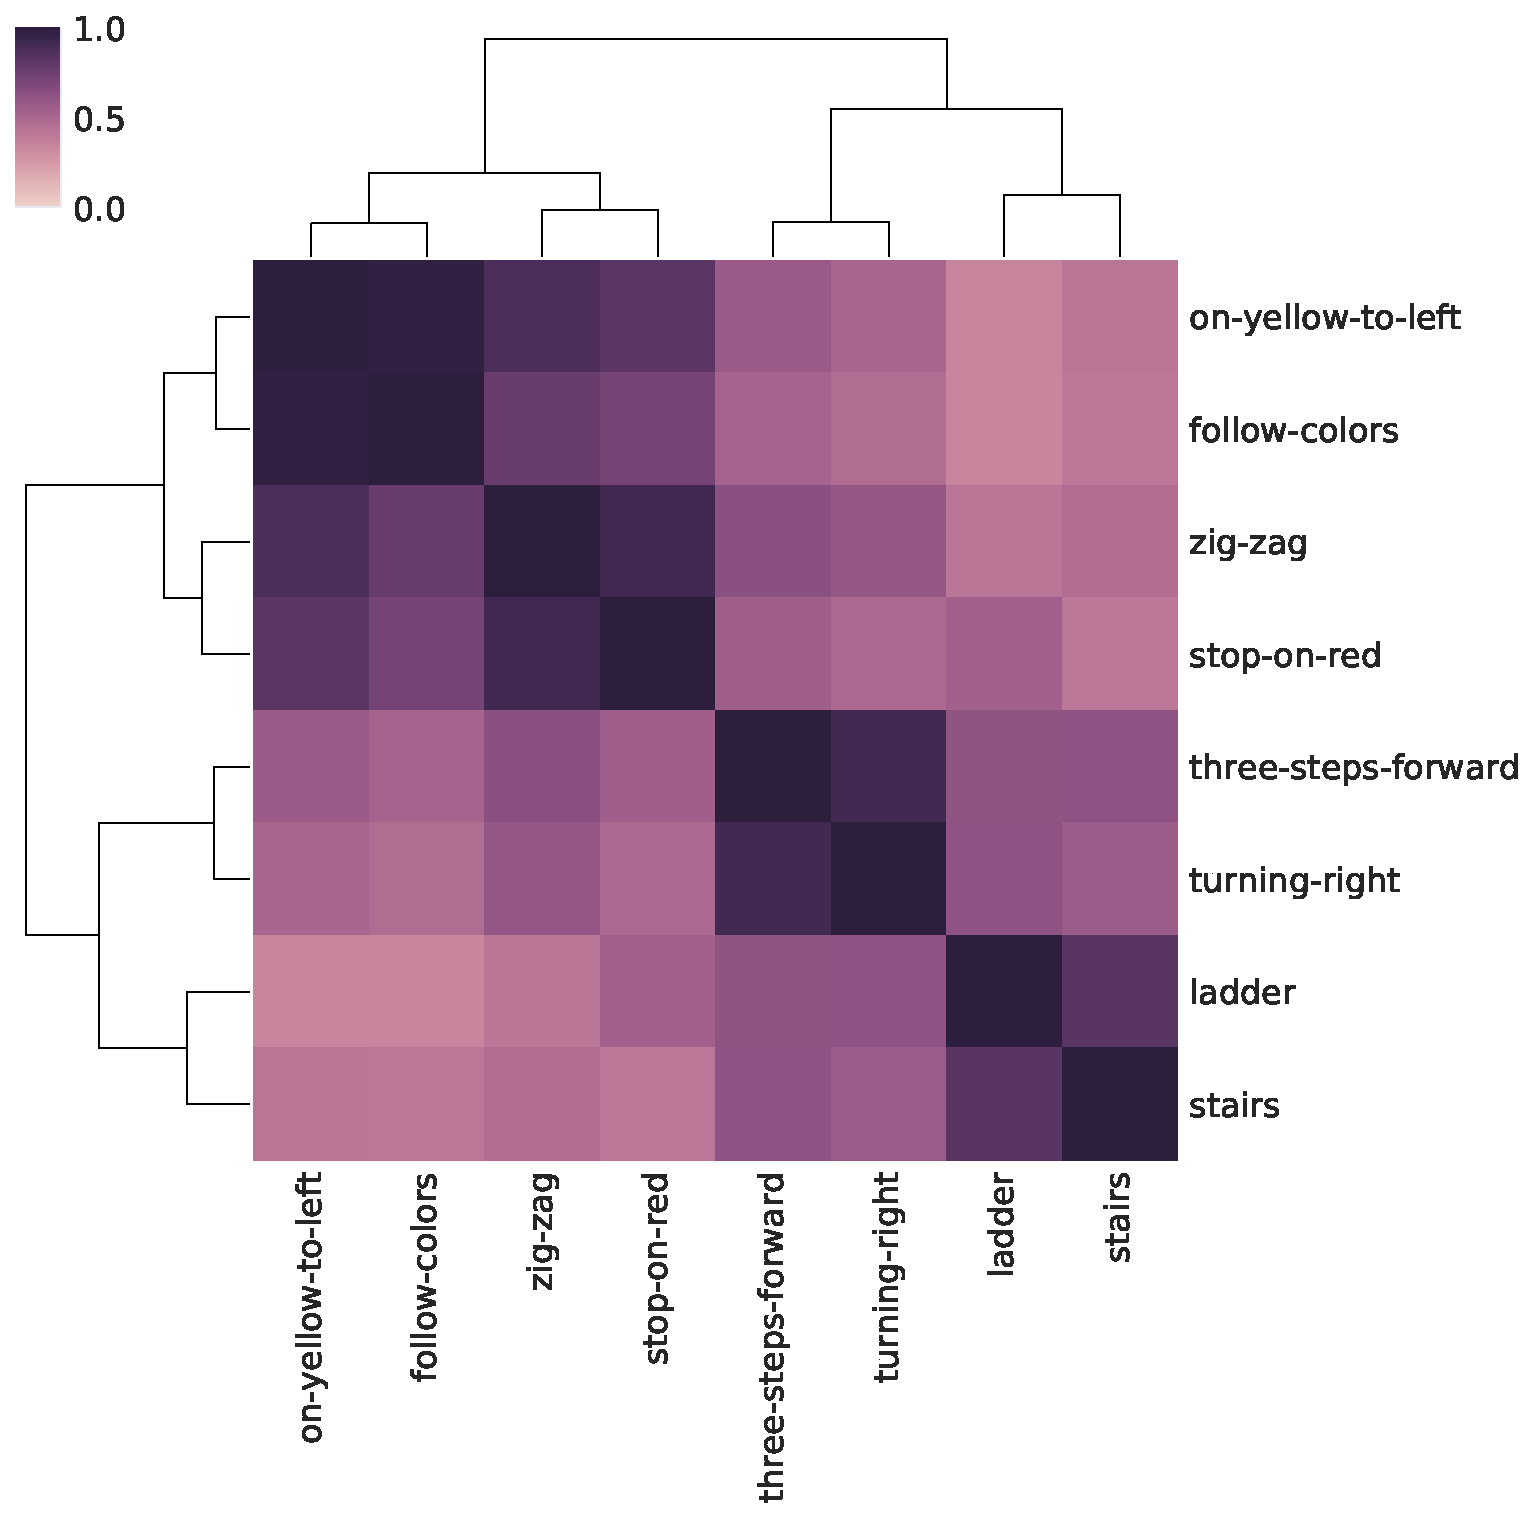
\includegraphics[width=0.48\textwidth]{img/similarities-tasks}
  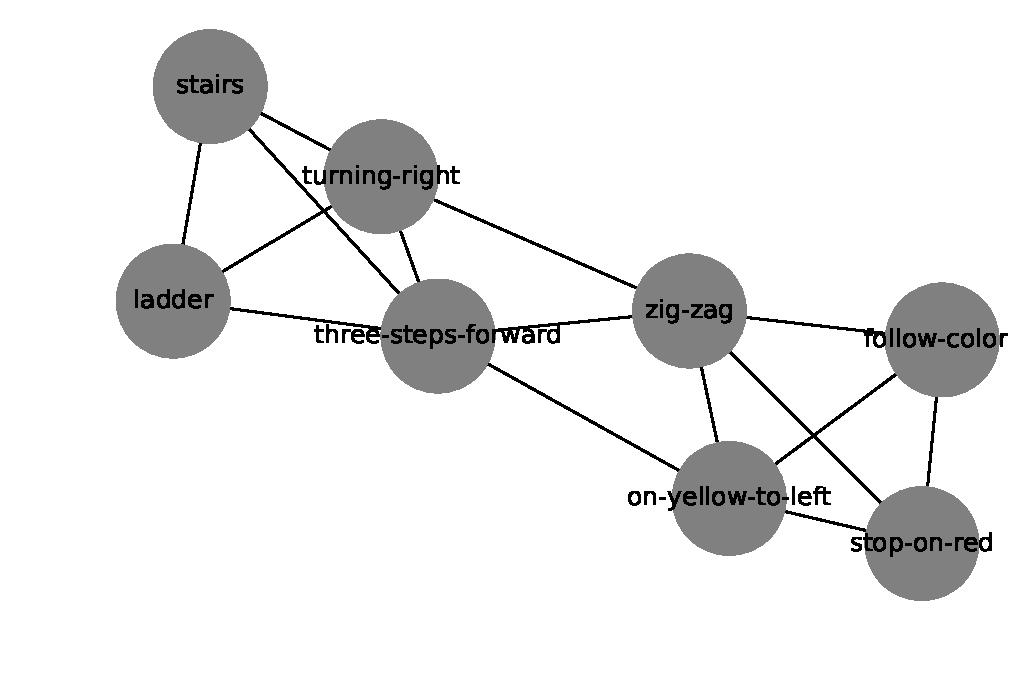
\includegraphics[width=0.48\textwidth]{img/similarities-graph}
\end{center}
\caption{%
  Left: Similarity matrix between tasks (TODO: how computed);
  right: Similarity graph with edges between tasks with high similarity.
  TODO: make it readable}
\label{fig:similarities-tasks}
\end{figure}




\section{Student Modeling}
\label{sec:student-modeling}

For the system to be adaptive, models of
  a student skill, task difficulty, and student-task interaction
  need to be designed, implemented, and evaluated using collected data.
The purpose of these models is to predict the probability that a given student
  would solve a given task
  and also the time the student would need to complete the task.

NOTE:
- comprehensive overview exists: \cite{its-learner-models, pelanek-learner-modeling}
- my goal here: how to choose and adapt the most common learner models for the domain
  of introductory programming

NOTE:
- restricted task/model (our focus): skill modelling
(broader models can also include affect (e.g. frustration, boredom), motivation, etc)

NOTE: hidden variables (hidden state) (knowledge and skills, possibly also affect, motivation)
vs. observable variables (correctness, solving time, time series of program snapshots)


NOTE - usage: by UI for showing feedback for the student, for tutoring model for detecting mastery and content (task/problem-set) recommendation, for online evaluation (insight for developers), offline evaluation (insigth by researchers and domain experts - teachers of elementary programmin)

NOTE: different models for different tutors,
here we will focus on models that can be used for mastery learning and task recommendation.


TODO: what is a student model formally?
prediction fn (student, task, domain, context, hyperparameters?) -> response of the student to the task in the context (for us, the response is mainly performance measured e.g. by solving time, but it can also include change in motivation etc.),
together with update rule (reducer fn): interaction -> student,
where interaction is 5-tuple (student, task, domain, context, performance)
(NOTE: not only for prediction for a performance on a task, also for
visualization skills in UI, providing feedback for teacher, etc.);
OR "offline student model": (domain model, complete history of the learner) -> prediction about the future behavior (vs. "online student model" with the update rule, more useful in our setting)

TODO: view from \cite{pelanek-learner-modeling}: data + procedures
- data: hyper parameters, population parameters, student skills
- offline procedures: parameter fitting -> metaparameters, population parameters
- online procedures: update equation, prediction equation

TODO: Student models vs. Domain models: (?) student models use domain as a
structure, assigning some parameters (e.g. skills estimate, uncertainty, or even
the full distribution of the estimate) to (some) "knowledge components" in the structure
- student models must by dynamic ("online") (i.e. parameters computed on the fly),
domain models can be possibly static (i.e. task and concept parameters can be computed offline),
example (from \cite{its-programming}): domain model is DAG of concepts together with a
Bayesian network over this DAG, ie. assignment of conditional probabilities to the edges;
student model: assignment from each concept to the knowledge (known / unknown / not-sure) -> knowlege for any concept can be then inferred using the Bayesian network
(? the Bayesian network is in this case same for all students, but does it make it part of the domain?)
- terminology:
  - concepts and tasks lives in the domain model and they can have corresponding
  concept skills and task performances in the student model
- view form \cite{its-learner-models}: domain model - state space, student model - state within the state spce
- domain model: offline (usually), student model: online (necessarily)



NOTE: categorization:
1. according to the underlaying domain model (-> single/multiskill, skills relationships etc.)
2. single point estimate / full distribution / sth. in between (e.g. mean and deviation=uncertainty)
3. online vs. offline (we need online)
4. according to the assumption about learning/not learning (we need to model learning)
5. (granularity? prediciting performance on concepts/tasks or even individual actions/ruleshigh-level skill tracing vs. fine-grained
6.,7. complexity; assumptions about learning \cite{pelanek-learner-modeling}
8. skill as discrete (BKT) or continuous (logistic models)




NOTE: modelling time vs. correctness/success
- time: log time (REF)
- corretness:
  - pure solved/not-solved (to coarse and no useful data - most students solve most tasks and if not, it is often because of reasons other than skill, e.g they need to finish the practice)
  - continuous partial credit - use response time (or even more detaild information about the task session) to map the performance to a correctness scale from 0 to 1 (see thran-thesis, p.106 for overview of tried mappings, e.g. expTime, thresholdTime, etc., but note that in MatMat they need to combine the time and corretness and this mapping is only done for correct answers),
  - discretized partial credit - (binary classification or 3 or 4 categories, e.g "poor", "good", "excellent" corresponding roughly to the 3-level flow classification: too difficult, just right, too easy)

NOTE: incorporating labor intensity of the item (e.g. into IRT, see thran-thesis, p.101)


NOTE: models without hidden states, e.g. based only and directly on observed performances
  (see knowledge space theory; relevant underlying domain model is AND/OR graph between
  tasks; using Markov chain for predicting student state)

NOTE: matrix-factorization approaches (e.g. Thai-Nghe et al. (2011))


TODO: \cite{student-models-review-2012}:
(for inner loop: cognitive tutors and constraint based models)
- cognitive tutors - skills as rules,
  mastered skill: rule correctly applied (multiple-times),
  allows for modeling misconceptions ("MISconcepts") (incorrect rules)
    -> useful for automatic hint generation ("just-in-time feedback"),
  example: the Lisp Tutor
- (and contstraint based modeling - skills as predicates)
- doesn't require long-term student model, can be just for the current topic;
  however, the transfer of skill estimates between topics can help,
  because 1 skill is often required in multiple topic
  - this is known as (\emph{transfer model} or) \emph{knowledge tracing}
  (and I think that it is the same thing which we call "prior knowledge estimation")
  (but in our context, \emph{skill tracing} would be better name)

Our focus is on the outer-loop as the inner-loop is better suited for people (instructors)
(REF: Essa, 2016: A possible future for next generation adaptive learning systems.)

NOTE on multiple skills:
Although modeling multiple skills seems useful,
  there is a trade-off between the complexity of the model (number of skills)
  and how well (or how fast) the parameters can be estimated.
More parameters require more data and time for the estimates to converge.
(and this is especially concern for students, because predictions are needed
immediately for new students (=no/little data) + students' skills are
assumed to change (tasks didn't have these problems).

\subsection{Data}
\label{sec:student-modeling.data}

To learn model parameters, such as difficulty of individual tasks, some data is needed.
What data and how much data is needed differs across models.
Some data about tasks are independent of students;
therefore, they can be obtained in advance,
which can be useful for initial task difficulties estimates.
Three types of task data are distinguished:

\begin{itemize}
  \item task statement (including name and world description),
  \item sample solution (or multiple solutions),
  \item expert labels (e.g. covered concepts).
\end{itemize}

Task statements are always available,
  because they are needed to present tasks to students.
However, obtaining sample solutions and expert labels
  incurs additional costs for a new system.
% TODO: Note that quite often, systems needs sample solutions and some labels
%       for the presentation purposes anyway.
Moreover, they can be noisy and imperfect.
For example, an annotator can forget to include some labels
  or even make a mistake in the sample solution.

Once the task is deployed in the running system,
  rich data can be collected from each interaction between a student and a task:
\begin{itemize}
  \item whether the task was eventually solved,
  \item solving time,
  \item number of clicks, number of code executions,
  \item program snapshots (e.g. after each code change),
  \item rating or labels provided by the student (e.g. perceived difficulty).
\end{itemize}

% TODO: also consider to include hints in the list
% TODO: mention different granularity levels for taking program snapshots (+cite)

\subsection{Item Response Theory}
\label{sec:irt}

The simplest version of item \emph{item response theory} (IRT)
  \cite{irt-visual-guide}
  models each student by a one-dimension skill $s$,
  and each task by a one-dimension difficulty $d$.
(NOTE: this special version is also known as one-parameter logistic model -- 1PL, or as Rasch model, ?, REF)

IRT assumes that the probability of a student with skill $s$
  successfully solving a task with difficulty $d$
  is given by the following function:
  \begin{equation}\label{eq:logistic}
  P(s, d) = \frac{1}{1 + e^{-(s - d)}}
  \end{equation}

% TODO: mention 2-parameter model (explain discrimination parameter)
\begin{figure}[h]
  \centering
  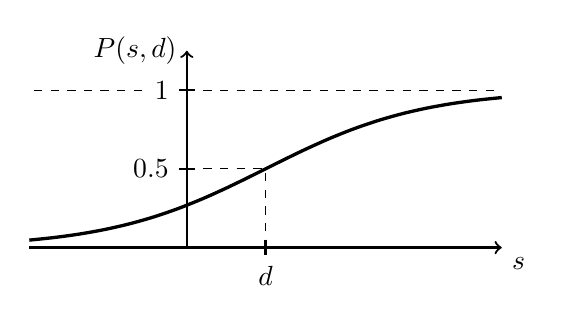
\begin{tikzpicture}[domain=-2:4, smooth, samples=20, scale=1]
  \draw [thick, ->] (-2,0) -- (4,0) node [below right] {$s$};
  \draw [thick, ->] (0,0) -- (0,2.5) node [left] {$P(s,d)$};
  \draw [thick] (-0.1,1) node [left] {$0.5$} -- (0.1,1);
  \draw [thick] (-0.1,2) node [left] {$1$} -- (0.1,2);
  \draw [thin, dashed] (0,2) -- (4,2);
  \draw [thin, dashed] (0,1) -- (1,1) -- (1, 0);
  \draw [thin, dashed] (-0.57,2) -- (-2,2);
  \draw [thick] (1,0.1) -- (1,-0.1) node [below] {$d$};
  \draw [very thick] plot (\x, {2 / (1 + exp(1 - \x))});
  \end{tikzpicture}
  \caption{One-parameter Unidimensional Logistic Model}
  \label{fig:logistic-model}
\end{figure}

NOTE: additional parameters: discrimination (how much is the performance sensitive to the skill), pseudo-guessing (the minimum probability of success, useful mainly for multple-choice questions, probably not very useful for us)

This basic model was originally developed for a simple knowledge testing
  and therefore it assumes a single constant skill.
However, programming skill is multidimensional;
  for example, one student can be proficient with functions and struggle with loops,
  while another student can master loops and struggle with functions.
Furthermore, these skills should be ideally changing significantly during
  the interaction with the system, because students are learning.

NOTE: multidimension extension: x = skill vector * discrimination vector - task bias
(this is basically what we tried in the first prototype, with fixed discrimination vector,
although we formulated it in the online "ELO" variant)
(REF?:The difficulty of test items that measure more than one ability.,
Using multidimensional item response theory to understand what items and tests are measuring.)

Another drawback of the IRT is that it only uses
  the binary data about successes and failures.
As nearly all interactions in programming learning systems end with a solved task,
  it would be more useful to work with solving times,
  which can provide more information about students' skills.

Item response theory can be extended to overcome these limitations.
\emph{Problem Response Theory} (PRT)
\cite{alg.problem-response-theory, pelanek-student-modeling-times}
% TODO: only cite the more relevant paper (or extend this section and cite both
% on relevant places)
predicts problem solving times instead of probability of success,
assuming an exponential relationship between a problem solving skill
and the time to solve a problem.
PRT can be formulated to use multidimensional skills.
The model parameters (skills and difficulties) can can be estimated from the data
  using one of the \emph{maximum likelihood estimation} algorithms.
  % TODO: cite paper describing the parameters estimation (or MLE?)
% (for IRT, it's \cite{irt-theory-and-practice}, but PRT would be better)

- underlying domain model:
  - single concept / flat concepts -> classical IRT
  - Q-matrix -> multidimensional version (see thran-thesis)
  - hierachical structure of concepts ? (see Millán and Pérez-de-la-Cruz (2002))

% TODO: find and provide the details about the learning extension of PRT
% (isn't it already the elo?)

% TODO: Add note that the assumption of exponential relationship is justified
% by observed solving solving times distribution and it is also intuitively
  % plausible - multiplicative nature of solving times.

NOTE: Main problem - without learning; in principle can recompute parameters after
each interaction, but that is not feasible in online learning systems; remedy: PFA (student-related parameters can be computed online,), Elo models (both student and task-related parameters can are computed online)

NOTE: IRT is a speical case of Naive Bayes, which is itself a special case of BN model:
  - Naive Bayes = all task performances are independent given the hidden latent skill
  - furthermore, the conditional probabilities P(performance on task t | skill
  theta) cannot be arbitratry, they must have a logistic distribution

NOTE: modeling response times (nice summary in thran-thesis)
- log-time from normaln distribution with mean d - a * theta (and variance c),
  ie. assumption is exponential relationship between the solving time and the skill?
  (this statement is not clear, because it depend on what you denote as skill,
  e.g. if you say that skill is exp(theta), than the relationship is linear...)
- incorporating multidimensionnal skills (flat concepts model): d, a vectors; update skill of each concpet contained in the task


NOTE: PFA - logistic model with learning (logistic fn, set of skills for each concept, initial skills, constant incread after a correct answer; total skill = sum of skills of concepts contained in the task, squashed byt the logistic fn)
REF: Pavlik 2009: Performance factors analysis—a new alternative to knowledge tracing.

NOTE: PFAE - combines Elo with PFA (make the PFA online for both student and task parameters)
(basic version: no domain, repeated answers to single item -> prior knowledge + current knowledge,
not sure how much relevant for us)



\subsection{Elo}
\label{sec:elo}

The Elo model \cite{alg.elo, irt-elo-math}
  extends the logistic model presented in section \ref{sec:irt}
  to capture changing knowledge.
Inspired by the rating of chess players \cite{elo-rating},
  the model interprets each attempt  to solve a task
  as a ``match'' between the student and the task.
After this match ends, skill and difficulty estimates are revised.

If the student solves the task faster than expected by the model,
  their skill is increased and the difficulty estimate of the solved task is decreased.
On the contrary, if the student fails to solve the task or if takes them too long,
  their skill is decreased and the difficulty estimate of this task is increased.

% TODO: formulas (for time-variant of elo)
% TODO: mention differnet updates for tasks (exponentially decayed) and
% students (their skill is assumed to change and not converge)

The main advantage of using the Elo model is its simplicity, flexibility,
  good performance and intrinsic online nature, which allows for immediate
  updates of parameters as students are interacting with the system.


NOTE: Elo variant based on network model: each time a task is solved, update skill for all tasks according to the similarity to the one solved (this can be propably also done on the level of concpets, if we have a similarity network between concepts)

NOTE: Elo variant for concept model ("simple hierarchical model" from thran-thesis),
as basic Elo but the total skill is the sum of the global skill and concept skill
(updating both the same way)

NOTE: Elo variant for hieararchical model:
- predictions: total skill = sum all ancestors skills
- update: all ancestors sequentialy (from the top-most), elo-like update

\subsection{Bayesian Knowledge Tracing (BKT) / Bayesian Networks}
\label{sec:bkt}

- BN:
  - underlaying domain model: BN (prereq DAG?) of concepts and tasks:
  - hidden nodes = skills of concepts (and misconceptions)
  - observed nodes = performance on tasks
  - edges = conditional probabilities of mastering given skill given that the
  parent skill is mastered; or that a task will be solved with given level of performance
  (skills are usually modeled as continous number, so this conditional probability requires
  either discretization or using/assuming? normal distribution for the skill estimate)
  - student model adds the oberserved performances and uses the Bayesian inference to
  predict performance of new tasks (? or is there a way to do equivalent online update
  and store the skills, so that no inference is needed (space-time tradeoff)
  - example: \cite{its-programming}.

- ? possibility to construct the BN from the observables (tasks) only -> makes the estimation
  more feasible as there are less hidden variables (it can be even constructed dynamically
  in each situation only from already solved tasks, so that all variables are either
  observed or query, no hidden ones)

- TODO: figure: note that BN encodes conditional independencies between concepts,
  so e.g. there must be "horizontal edges" between phases of a mission,
  because a phases are not independent given a mission skill;
  (the figure should include not only problem set chunks, but also an example
  of a cross-concept, e.g. loops, and possibly game concept, e.g. wormholes)

Pros:
- rich model
- intuitive graphical representation
- mathematical derivation for the inference

Cons:
- requries to set the domain structure by the expert (there are some mothods for finding the structure, but that requires a lot of data)
- requires a lot of data to reliably estimate the conditional probabilities
- ? exact inference probably not possible (big network + continous distributions),
  so it requires approximate inference (? sampling techniques)
  vs. online tracking of skills (online update)

TODO: Xu, Y., Mostow J.: Using logistic regression to trace multiple subskills in a dynamic Bayes Net.

TODO: Wang et al. 2013: Dynamic item response theory models
(combining BN with logistic models)

\subsubsection{AND-OR Bayesian Network}

TODO:
- based on \cite{student-models-review-2012} (section 5.1.2)
- move releavntk part to domain models section and ref it
- what it is: assumption on the conditional probabilities to make the inference feasible?
- two type of nodes: Leaky-OR, Noisy-AND:
  - OR: single mastered parent concept is enough to master the child chunk (task/concept)
  - AND: all parents need to be mastered to master the child chunk
  (? orientation of edges in this context is not clear to me: in our hierearchy,
  I think it make sense to have parents depend on children, e.g. mission on
  phases (AND), phases on tasks (OR))
- ? at least in the basic formulation, having multiple parents for the OR node doesn't help
  at all, same for having all but 1 parents of AND node mastered, that seems too limiting...
- related terms: NIDA/DINA, NIDO/DINO models


\subsubsection{BKT}

- Dynamic Bayesian Network - Bayesian network with time (each variable also
  depend on itself in previous timestep (genearization of HMM)
- BKT = special type of DBN (even HMM at least in the basic form, for single skill):
  for each skill, two hidden states (known/mastered) or not,
  observed: variable: performance
- assumes: learning (in contrast to basic IRT), discrete knowledge state (eithter known or not known)
- assumes: on each opportunity to use the skill (e.g. solving a task with the corresponding concept), there is constant probability of learning that skill
- TODO: add the standard diagram of BKT (possibly for some relevant extension, such as multiple skills?)
- many extensiosns (...), TODO: describe an extensions relevant for us:
1. hiearchical model of skills (as used in the current domain model)
2. DAG of concepts, DAG of tasks with imposed Bayesian network
- TODO: parameters estimation (both the "domain parameters" and "student parameters")

TODO: BKT with time: Leveraging first response time into the knowledge tracing model.


\section{Tutor Models}

(ordered from the most outer to the most inner loop)
- content sequencing (curriculum sequencing) (\cite{its-programming}) (which topic to do next?)
  (this is relevant for the systems with a lot of content, not our case -> not our focus)
  (focus on prerequisities so that from evidence about one skill, say nested loops, can
  infer that many other skills are mastered, e.g. sequences, single loops, conditions)
  (term: "learning path")
- mastery learning (Umime programovat) (continue with the current topic or progress to the next?)
- task recommendation (Tutor) (which task to solve next?)
- "problem solving / solution analysis / solving process tutors",
  (e.g. cognitive tutors, constraint based models)
  (which step to do next towards solving the task? -> which hint to show?)

- hierarchical tutor: using different student models for different loops
  (inner, outer curriculum)

\subsection{Task Recommendation}
\label{sec:task-recommendation}

Student models are used by an \emph{instructional policy} to recommend
  the most suitable task for a student.
In spite of having all the predictions about success probabilities
  and time estimates available,
  task recommendation is not an easy task.
First, it is not clear what difficulty level is optimal.  % TODO: example (75 % of success etc.)
Second, it may vary for different students, domains or types of problems.
Furthermore, optimal difficulty is not the only criterion to be considered.
For instance, diversity of tasks is important to keep students interested.
No principled techniques for task recommendation have been developed yet;
however, several heuristic approaches have been used
  and proved to work well (TBA: ref).

TODO: clarify terminology:
- instructional policy (not defined!) vs. tutoring model (same?);
- outer and inner loop (figure?)
  (outer loop: "problem selection loop", "macroadaptivity",
  choosing chunk, choosing a task within a chunk,
  inner loop: "microadaptivity", "problem solving and solution analysis tutors"
  - helping a student to solve the task, giving hints, providing feedback).
  (\cite{its-learner-models}: inner = problem step, outer = problem selection,
  curriculum loop = which chunk)

Task recommendation is not a necessary requirement
  for the system to be adaptive.
Student models can be utilized by other means to achieve personalized behavior,
  e.g. in mastery learning (section \ref{sec:mastery-learning}).
The system can also just provide students with predicted solving times
  and let them to choose the next task they want to solve.

Showing predictions can be already perceived as a very mild form of recommendation.
Indeed, recommendations can range from \emph{soft} to \emph{hard}.
Soft recommendations can be achieved either by
  ordering tasks according to suitability,
  filtering and only showing a subset of tasks,
  or showing suggestion such as
  ``too easy'', ``too difficult'' and ''ready to attempt'' next to each task.
For example, suggestions in the form of traffic-light colors
  are used in the system described in \cite{its-programming}.
The system can be more strict and show only a single recommended task,
  or even enforce the recommendation by immediately progressing student to
  the next task without asking and giving them a chance to select a different task.

\bigskip
\emph{TODO:\\details about techniques (heuristics, methods) for selecting single best task}

% TODO: mention simple heuristic approach from Tutor: 2 tasks of similar difficulty as the just solved task which were not solved previously

\subsection{Mastery Learning}
\label{sec:mastery-learning}

\emph{TODO:\\describe mastery learning + usage of student models%
(to show the progress and to determine that the student already achieved the mastery)}

- what it is: type of instructional policy (tutoring model); practice of a topic until covered concepts are mastered, only then move to the next topic

- what is needed: online algorithm for deciding mastery given a stream of s-t interactions ("mastery criterion")

- how: basic version: compute a simple summary statistic such as average
success or number of correct answers in a row and compare with a threshold;
instead of a simple summary statistic, a student model (section
\ref{sec:student-modeling}) can be used (e.g. predicting probability of success
or a fuzzy skill of given concept)
(DQ: it seems to me, that a simple summary statistic is just an extreme case of
a student model; or is there a fundamental difference? E.g. making or not
making an assumptions about learning, as (implicitly) suggested in \cite{alg.mastery}?
Or being able to predict some sort of performance of the student, e.g. probability of
success?)
(REF same examples using student models, see \cite{alg.mastery} for relevant
papers to read)

- examples of systems using mastery learning (ref to the previous chapter)

- important: which data to use for decision (specifically: it is important to
incorporate solving times); concerning the technique, EMA (exponential moving
average) is sufficient; modeling students does not result in a significant
improvement \cite{alg.mastery}

- usage of response time:
1) discretization, but binarization is too coarse
-> notion of partial credit, e.g. 1 for fast solution, 0.5 for slow solution,
0 if failed to solve;
2) continuous mapping from respone time to the 0-1 range
(e.g linear fn from 0s to 2*median secs, then 0 \cite{alg.mastery})


- choosing the right threshold (balance between overpractice and underpractice;
(application dependent));
- ? using effort-score graphs \cite{alg.mastery}
- ? require the maximum time to achieve the mastery for genius

% "fixed outcome, varied time" (vs. classical education: fixed time, varied outcome)

% TODO: screenshot of a mastery progress bar (e.g. from UmimeX)

\subsection{Adaptive Scaffolding}

TODO: terminology:
  scaffolding (broader term, not necesarily just-in-time or automatic),
  "just-in-time feedback" (\cite{student-models-review-2012})

TODO: maybe just mention in the intro

TODO: automatic hints /explanations / instructions / worked-out example selection/generation,
  (or suggestion to try easier task)


\section{Metrics and Evaluation}
\label{sec:metrics-and-evaluation}


To decide if the adaptivity improves the quality of the learning system,
  suitable metrics must be chosen and evaluated.
Metrics are also used for optimizing models,
  first for parameters fitting, second for choosing hyperparameters,
  and third for selecting best model from a set of possible models.

%TODO: table/diagram showing goals hierarchy and their usage:
%1. mission -> guide for long term objectives? (not measurable)
%2. long term objectives -> AB experiments
%3. live evaluation -> spot problems ASAP
%4. offline evalution -> learn hyperparameters; holdout evaluation
%5. guide learning -> to optimize model (learn parameters, incl. only updates after new s-t interaction)

\subsection{Mission Statement}
\label{sec:mission}

There are hundreds of possible metrics that the system could measure.
What metric to choose depends on the purpose of the evaluation,
  which can range from guiding a parameters-fitting algorithm
  to interpreting results of an AB experiment.
To make sure that chosen metrics are not misleading,
  they should reflect the ultimate goal of the system,
  which is sometimes also called the \emph{mission}.

Even the mission itself should reflect some higher-level goals.
Nevertheless, goals create an infinite hierarchy
  and a starting point (called \emph{paradigm}) must be chosen,
  from which the lower-level goals are derived.
An example of such paradigm is
  ``effort to maximize the overall happiness in the population''.
% TODO: Without going into further philosophical discussions or attempts for precise definitions,
%       ... we will just adopt this paradigm for the rest of this thesis.

At first sight, a reasonable mission of a system for learning programming
  is a long-term increase in algorithmic-problem solving skill in the population.
However, other factors than the skill should be considered as well.
For example, how much students enjoyed the time in the system,
  how they are satisfied with their accomplishments,
  or if they are motivated for further learning of programming;
  all of these may play an important role for the overall happiness in the population.
In the \emph{Rules of Machine Learning}, Martin Zinkevich
  points out that there is no single best objective \cite[][Rule \#39]{google-ml-rules}.
As a solution to this ``multiple objectives dilemma'',
  the mission can be formulated as achieving a balanced increase in all
  of these important factors.
Such formulation reminds developers of the system not to overfocus on one factor
  at the cost of the others.


\subsection{Long Term Objectives}
\label{sec:long-term-objectives}

The huge disadvantage of the mission statements
  is that they are not measurable.
To make informed decisions,
  such as which of the two recommendation algorithms to prefer,
  measurable metrics are needed.
Therefore, various proxy metrics are used.
These proxy metrics should be precisely formulated and measurable,
  but at the same time they should be related as much as possible to the system mission.

To elaborate on the mission from section \ref{sec:mission},
  a long term objective could be
  ``maximizing the number of students
  who mastered elementary programming quickly while having fun''.
To make this metric usable,
  terms ``mastering elementary programming'', ``quickly'', and ``having fun''
  must be defined in a measurable way.
While ``achieving mastery in elementary programming quickly'' can be
  formulated as an objective criterion
  (e.g. ``the student solved at least 5 tasks for each concept, each in less than 5 minutes''),
  ``having fun'' requires the system to ask students about their subjective feelings.
% TODO: note that looking at the mission statement above,
% it's not clear that there must be an objective mastery criterion
% which should be achieved by all students

Furthermore, a time frame must be specified, for example last 30 days.
While short time frames allow for faster decisions and hence more improvements over time,
there are several reasons for making the time frame longer:
\begin{itemize}
  \item to collect enough data for statistical significant results,
  \item to avoid seasonality effects (such as different user behavior during weekends),
  \item to allow for more exploration, which improves long-term performance of the system.
\end{itemize}

There are many other possible long-term metrics, for example:
\begin{enumerate}
  \item Daily active users (DAU) -- students who have solved at least 1 task this day.
  \item Monthly number of active users (30DAU) -- students who have solved at least 10 tasks this month.
  \item Returning users -- students who have solved at least one task one day and have returned and solved another task another day.
  \item Converted users -- students who have finished last level in the system.
  \item Converted users -- students who have solved at least one task from each level.
  \item Number of solved tasks.
  \item Total time spent on successful attempts.
\end{enumerate}

It is not immediately clear which of these metrics is the best proxy for the system mission.
Thankfully, it was observed that at the beginning all the metrics which seem to somehow
reflect the system mission tend to improve simultaneously, no matter which one
is chosen to be directly optimized \cite[][Rule \#12]{google-ml-rules}.
To understand how their values are influenced by changes in the learning system,
it is useful to measure and report all of them from the beginning
\cite[][Rule \#2]{google-ml-rules}.

All of these suggested metrics measure a complex aggreage effect of the system
behavior during some period.
However, it is recommended to start the system optimization with a metric which is simple
and directly attributable to individual recommendations \cite[][Rule \#12]{google-ml-rules}.
The attributable metrics are presented in section \ref{sec:live-evaluation}.

% TODO: diagram of A/B testing, e.g. https://receiptful.com/blog/ab-testing-for-ecommerce
% TODO: note on AB experiments: there will be always a difference -> needs to asses statistical significance (is the difference due to changed condition or just because of random noise)
% -> t-test and similar (but mind their assumptions!) -> p-value + alpha-level -> decision
% -> add error bars to measured metrics: e.g. 95% confidence interval / standard error / standard deviation / range (+ effect size)

\subsection{Evaluation of Programming Skill}

% TODO: dichotomy between enjoyment and learning metrics - enjoyment is easier to measure (length of interaction), but learning is possibly even more important for the system mission (neither pure enjoyment nor pure learning would work -> principle of balance); measuring enjoyment -> survival analysis; measuring learning -> learning curves
% TODO: for measuring learning in AB-experiments: (pretests) and postests

The tasks environment in the learning systems usually differs significantly
  from the real-world environment,
  e.g. by using block-based programming language,
  or by other aspects mentioned in section \ref{sec:strategies-for-easier-learning}.
Ultimately, what matters is the performance of students in the real world,
  outside the simplified learning environment%
\footnote{%
  This issue is also mentioned by Weintrop and Wilensky %
  in \cite{challenges-of-blocks-based-environments}, %
  in the context of proper evaluation of block-base programming environments.}.
This aspect should be considered when choosing a proper long-term objective.
For example, trying to achieve minimum solving times on tasks in the learning system
  might be a misleading objective
  -- it would likely lead to ``overfitting'' students to the particular learning system,
  by giving them all available tasks from the simplest to the most difficult.

TODO: REF 5-week high-school experiment, block-based vs. text-based:
- \cite{comparing-blocks-text-weintrop2017}
(important feature for such comparision is to have a two learning environments,
that only differ in the text/block version of the editor, everything else being same).


\subsection{User-centered Evaluation}

In addition to quantitative (objective) metrics (such as whether the
recommended task was clicked and solved), the system can also explicitly ask
students to provide qualitative (subjective) feedback.
For example, after the student solves the task, the system can show a dialog
asking about the perceived difficulty -- whether the task was ``too
easy'', ``too difficult'' or `just right''.
Other tags about tasks can be collected as well, e.g. ``boring'', ``weird'', or ``fun''.

Collecting these tags allows to compute metrics that looks as close proxies to
the system mission, such as the total time spent in flow.
As it combines both enjoyment and learning,
flow would be a great proxy if it could be measured reliably.
% TODO: ref to a relevant research about flow

However, a known disadvantage of subjective ratings is the amount of noise
in them. They are significantly influenced by the current mood and attention of
the student.
In addition, answering these questions may bother students a little bit
and it also takes some time the students could spend on learning instead,
(but it is negligible compared to the practicing time).

TODO: quantitative vs. qualitative and online vs. field studies are othogonal,
all combinations possible: e.g. in the field study \cite{comparing-blocks-text-weintrop2017},
they measured both quantiative data (performance) and qualitative (attitude);
the same can be done in the online learning system.

TODO: note on other user-centered evaluation strategies:
questionaires, free feedback (via feedback button), user-testing (single student / class), focus groups, semi-structured interviews with sutdents.

TODO: example of a 5-week experiment in schools (field study):
\cite{comparing-blocks-text-weintrop2017}
- investigated qualities: confidence, enjoyment, perceived difficulty, interest in future opportunities to learn CS, authenticity of the environment - "is it similar to what real programmers do?", efficiency of the environment ("made me a better programmer?")

TODO: example of short user study asking for perceived quality of recommendations
(of remedial tasks) \cite{learner-models-integration-skills}

\subsection{Live Evaluation}
\label{sec:live-evaluation}

In some learning systems, a new version of a model is deployed every day
  with parameters learned from the recent data.
The behavior of the new model must be carefully monitored
  to detect problems as soon as possible,
  without waiting several weeks to evaluate an AB experiment.
For this purpose, metrics that can be linked immediately
  to the recommender actions are needed.
These metrics are called ``online attributable metrics''  % TODO: find used terminology
and this type of evaluation ``live evaluation''.

These metrics are often formulated as a question concerning a single recommendation.
To transform them into a number, either sum or average of these individual errors is computed.
% TODO: so sum or average? or some other aggregation function?

Reflecting the long-term objectives from section \ref{sec:long-term-objectives},
  there are some examples of online attributable metrics:
\begin{itemize}
  \item Was the recommended task chosen by the student?
  \item \ldots and did the student solved the task?
  \item \ldots in a reasonable time (e.g. 1-15 minutes)?
  \item \ldots and did not the student marked it as ``too easy'' or ``too difficult''?
\end{itemize}

% TODO: relationship to metrics defined in section \ref{sec:metrics-for-recommendation}

% TODO: note on online models (and relation to RL), these needs continuous online evaluation

% TODO: taking delta wrt. previous model


\subsection{Offline Evaluation}

Offline experiments use historical collected data
  to avoid the cost of live evaluation.
The advantages of offline experiments compared to online evaluation include
  the possibility to run as many experiments as needed,
  obtaining the results quickly,
  reusing the same data to evaluating different models,
  and avoiding potential negative impact on students if the evaluated model is poor.

Of course, offline evaluation is limited,
  because there are not all the historical data needed
  for proper evaluation.
For example, when evaluating a new recommendation algorithm,
  the data about a student responding to a particular recommendation
  are often not available.
Another disadvantage of offline evaluation compared to live evaluation
  is that the data used for evaluation does not come from the completely
  same distribution of events as will occur in the live system,
  which limits generalization guarantees of such evaluation.
% TODO: note: further decrease of relevance to the system mission - but worth

Offline evaluation is typically used as a check before pushing
  the model online to avoid problems as soon as possible.
It can also be used for model selection,
  including hyperparameters search.
Finally, offline learning algorithms typically also use
  a metric to guide them
  (these are discussed in section \ref{sec:metrics-to-guide-learning}).


TODO: comparing to other (e.g. currently used) model (e.g. correlation between predictions, delta between recommendations):
1. for a prototype (idea) of new model: if the correlations are high, there is probably no significant gain in exploring this model (compared to using the current one);
2. for same model with retrained parameters for newly collected data - if the delta is too big, we should be suspicious and investigate.

TODO: evaluating parameters stability (see thran-thesis) - as above just with the same model (comparing the same model trained on different samples from the collected data)

\subsection{Cross Validation}

TODO: consider removing this section and only point to a relevant description
of CV in the context of student models evaluation, e.g. in \cite{pelanek-learner-modeling}
(our main scenario/methodology: "online evaluation with generalization to new learners")

Trained models must be evaluated on data unseen during training.
Straightforward approach is to split collected data into two parts,
  first used for training (\emph{training set})
  and second for evaluation (\emph{test set}).
To use data more efficiently, the train-test split can be repeated
  $k$ times, taking different $1/k$ portion of the data for testing every time,
  and computing averaged performance.
The described method is called \emph{cross validation}.

While random train-test split over all training examples works often
  best in many machine learning domains,
  one must be careful when dealing with data from learning systems.
A completely random split would lead to predicting past performance
  of student from the model trained on their future performance,
  which could result in over-optimistic results.
The recommended splitting technique is ``user-stratified'',
  in which we randomly split students,
  and create training set from all events of one group of students,
  and first $n$ events of all students in the second group.
The test set then contains $(n+1)$-th events from the students
  in the second group.
The evaluation can be repeated for all possible $n$'s and averaged.
This is simple and fast for online models
  (that can be trained iteratively by one training event),
  but it is more involved and often too slow for offline models.
To make the evaluation reasonably fast,
  some simplifications can be used,
  such as predicting not only one, but multiple events
  for each student in the second group during a single split.

% TODO: make it clear that even for online models, we are still discussing offline evaluation
% TODO: discuss compromises for evaluation of offline models (or point out to a relevant paper)

If the model contains hyperparameters to select,
  it is important to use yet another non-overlapping portion
  of data for hyperparameters search,
  which used neither for training, nor for final evaluation.
This third portion of data is sometimes called \emph{validation set}
  (though the terminology for this is not unified).
Cross validation can be generalized to account for this 3-parts split
  and the resulting method is called \emph{nested cross validation}.

% TODO: figures to illustrate all the described methods and splits

NOTE: \cite{student-models-review-2012} also discusses the "correct level on
which to perform the cross-validation": never on the level of individual
"actions" (task sessions), but rather on the student level (to see how the
system will behave for the new students in the system, for which it wasn't
pretrained offline), sometimes it make sense to use the "chunk level"
(to see how it generalizes to new chunks), "school levels" (new populations of
students)
(in sklearn this is called "Group k-fold cross-validation")

\subsection{Student Model Evaluation}
\label{sec:student-model-evaluation}

A student model (described in \ref{sec:student-modeling})
  is an important component for adaptive learning techniques
  such as recommendation algorithms.
Therefore it is reasonable to believe that optimizing the quality
  of used student models should result in better recommendations
  and transitively in improving the long-term objectives.
Although better predictions usually help,
  the relationship between their quality and the long term objectives
  is not always straightforward.
If the online experiments show that the more accurate predictions would actually
  lead to decrease of the long-term objectives,
  then these improvements in the predictive power should not by applied.

The next two sections present metrics for two most common
  types of student models according to their output:
  predicted solving times and predicted success.
% TODO (consider): generalize: any real values (e.g. times)
%                  vs probabilities (success, too-difficult)


TODO: Student models are used for different purposes
(e.g. inner loop, outer loop (task recommendation) human-in-the-loop (insight),
open learner visualization, )
evalution should reflect the intended purpose
(see \cite{pelanek-learner-modeling}).

NOTE: overview of metrics for student models comparison, e.g. in \cite{pelanek-evaluation-student-models}

TODO: reliability and resolution of predictions (also in \cite{pelanek-evaluation-student-models})

TODO: reliability/stability of parameters

TODO: "plausibility of parameters" \cite{learner-models-integration-skills}


\subsection{Metrics for Time Predictions}
\label{sec:metrics-for-time-predictions}

% TBA: note on data we need (and easily collect in this case)
To evaluate the quality of solving times predictions,
  vector of predicted times $\hat{t}$ is compared to
  the vector of true observed times $t$.
Usually, individual errors between tuples $(t_i, \hat{t}_i)$ are computed
  and then averaged.
While it is possible to take an absolute value of the
  difference $(t_i - \hat{t}_i)$,
  which results in Mean Absolute Error (MAE),
it is more common to taking square of the difference
  to penalize more one large error than multiple small ones.
In this case, it is common to take a square root of the final
  average, to bring the units back to the original ones
  for better interpretation.
This metric is called Root Mean Squared Error (RMSE).

$$
RMSE(t, \hat{t}) = \sqrt{\frac{1}{n} \sum_{i=1}^n (t_i - \hat{t}_i)^2}
$$

Note that the solving times should be first log-transformed;
  otherwise a single outlier could make the error extremely high.
% TODO: provide more details/ref to an earlier section about taking logs
% TODO: also note that these type of metrics will be always susceptible to
% outliers anyway

% TODO: Statistic notes why the RMSE makes sense:
%       - explain that given some assumption
%       -> results in best linear estimator
%       - and even MLE (assumption of normally distributed noise),
%                       -> it's equivalent to RMSE - see Bishop, 2006)

%TODO: The metrics presented in this section
%  can be also used for evaluation of other real-valued predicted variables,
%  such as flow (if formalized to take real values.)


\subsection{Metrics for Success Predictions}
\label{sec:metrics-for-success-predictions}

Some student models predict a probability that
  a given student would solve a given task.
% TODO: statistics terminology - alternative distribution
In this case, each the true labels are not any real number,
  but just zeros and ones.
This difference is important for the choice of a suitable metric.
Good overview of possible metrics is presented in \cite{pelanek-evaluation-student-models},
  which also shows a simple example demonstrating why MAE should not be used
  as an error measure for binary predictions.
In addition to RMSE, Log-Likelihood (LL) is sometimes used:
$$
LL(s, \hat{s}) = \sum_{i=1}^n s_i\log(\hat{s}_i) + (1-s_i)\log(1-\hat{s}_i)
$$
% TODO: include derivation of LL from MLE principle (product -> log -> sum)
Note that LL differs from RMSE in several aspects.
First, as opposed RMSE, the higher LL the better,
second, it is negative,
and third, it is not averaged, so it decreases with the size of data set.

The RMSE and LL are based on a probabilistic view of errors.
There is another set of metrics based on the qualitative understanding of errors,
  which compares the observed success with binarized predictions,
  instead of real-valued probabilities.
For example, \emph{accuracy} is a ratio between correct predictions to all predictions.
However, these metrics do not distinguish between small and large errors of the predictions,
  which makes them less appropriate for student modelling.

% TODO: details, possibly table of common metrics from the confusion matrix
% (precision, recall, sensitivity, specificity, ...)
% TODO: mention: allows for setting different risks (weights) on different types of errors
% TODO: diagram: comparison of these individual errors, see pelanek-evaluation-student-models, p.6

These error metrics depends on a particular threshold chosen
  for binarization of predicted probabilities.
There are metrics avoiding this problem by using only ranking of predictions.
The most common one is AUC, ``Area Under Curve'',
  which is the probability that if one failure and one success are selected by random,
  the predictor would assign a higher probability to the success event than to the failure.

There are a few limitations of AUC.
First, it considers all thresholds, but only a range of them is usually relevant.
Second, by only considering the ordering of predictions,
  if all predictions are multiplied by a constant, AUC remains unchanged.
Third, if the predicted classes are strongly imbalanced,
  high AUC can be achieved by simple classifiers
  even if they perform poorly on the minority class.
Generally, AUC is a reasonable choice for intrinsically classification problems,
  but not necessarily for student modeling \cite{pelanek-evaluation-student-models}.

% TODO: precise definition of AUC using ROC curve
% TODO: check if the intuitive explanation of AUC is correct
% TODO: how to deal with the limitations: global objectives (ranges of thresholds), AUC-PR for unbalanced problems

\subsection{Offline Evaluation of Recommendations}

% TODO: consider moving before metrics for predictions?

Offline evaluation of recommendation algorithms is considerably more difficult
  than evaluation of student models.
The reason is missing data --
  if the evaluated algorithm recommends a task $t$ to student $s$
  in a specific point of his learning process (e.g. after first 2 solved tasks)
  but the student $s$ attempted different task at that point,
  there is no easy way to tell if the recommendation is good or not.

The extremeness of data sparsity makes offline evaluation so challenging,
that most learning systems completely skip this type of evaluation,
apply offline evaluation only to student models
(section \ref{sec:student-model-evaluation})
and check quality of recommendation algorithms on live traffic
(section \ref{sec:live-evaluation}).

Nevertheless, realizing that the offline evaluation serves just as another proxy metric,
  it may be still useful to perform at least some limited offline evaluation
  before putting the recommender to the wild of real world.
There are some possible approaches:
\begin{itemize}
  \item For each recommendation event in the collected data,
      look if the recommended event is among one of top $N$ (e.g. 10) tasks
      recommended by the evaluated recommender
      and compare it with the observation whether this particular recommendation
      was good (e.g. whether the student attempted and solved this recommended task).
      (These comparisons can be turned into several different metrics,
       which are described in section \ref{sec:metrics-for-recommendation}).
      % TODO: point to a section with confusion matrix, precision, recall etc.
  \item Instead of looking at the past recommendations,
      events when students themselves selected a task from a list of all tasks can be used.
      (It is also possible to combine both recommendation and self-selection events
       as a single dataset.)
  \item Prepare a small manually labeled dataset describing appropriate and
    inappropriate recommendations for given combination of features, possibly
    by extending collected data on recommendation.
  \item Measure agreement in recommendations between a new recommender and one which is already used and was evaluated on live traffic (recommended by \cite[][Rule \#24]{google-ml-rules}).
\end{itemize}

% TODO: note on data bias in most of these approaches

\subsection{Evaluation of Mastery Learning}

TODO: Effert vs. Score plot/metrics \cite{learner-models-integration-skills}

\subsection{Metrics for Recommendations}
\label{sec:metrics-for-recommendation}

There are multiple metrics that can be used for both online and offline
evaluation of recommendations.
These metrics can be divided into several categories
according to what data they need.

For a series of student-task interactions paired with a recommendation list of
fixed length $N$, a \emph{confusion matrix} can be constructed by comparing
whether the interaction was beneficial for the student or not,
and whether the task was within top $N$ recommended tasks.
Having the confusion matrix allows to compute various metrics such as
accuracy, precision, or recall. % TODO: or sensitivity/specificity/... + define

Depending on the user interface, fixed $N$ might or might not make sense.
If not, it is possible to use more sophisticated metrics without a fixed $N$,
such as AUC (described in section \ref{sec:metrics-for-success-predictions}),
or MAP (Mean Average Precision).
% TODO: MAP = AUC-PR?
% TODO: or DCG?

In some cases, for example when comparing two recommendation algorithms,
complete lists of ordered tasks are available.
In this case, other \emph{ranking metrics},
  such as Spearman's rank correlation coefficient,
  or Kendall's rank correlation coefficient,
  can be also used.
% TODO:  Discounted cumulative gain, average precision, lift index, ...

%# Beyond simple accuracy
All these metrics focus on accuracy of the recommendations,
but there are other properties of recommendation algorithms,
which may influence its usefulness for students,
such as robustness or diversity.
% TODO: note: but they are more difficult to express/measure,
% so they are used much less in practice

For example, if the system shows several recommended tasks,
but these are all nearly identical, there is no added value
for the student from the possibility to choose from them.
Similarly, if the student has just solved a task
without any problem, the next recommended tasks should
differ considerably not to be boring for the student.
To measure similarity between tasks, their content features
constructed from their statement and solution are compared
using some distance metric.
% TODO: ref to our current item-similarity research


\subsection{Metrics to Guide Learning}
\label{sec:metrics-to-guide-learning}

Learning algorithms often incorporate a metric they attempt to optimize.
In this context, the metric is often called \emph{loss function}.
For example,
  Ordinary Least Squares (used for linear regression models) minimizes RMSE.
Some learning algorithms, such as gradient descent,
  allow to minimize arbitrary metric
  for which it is easy to compute partial derivatives with respect to model parameters.
Loss functions can be viewed as just further proxies for long-term objectives.
Therefore, in the case of choice, it is beneficial to choose a loss function
  that matches the long-term objectives more closely.

As a common example, some loss functions allow to specify weights for each training example.
If it is derived from the long-term goals that predicting one class correctly
  is more important than predicting the other class correctly
  (e.g. if it is more important to predict correctly failure than success),
  larger weights should be assigned to the examples with the more important class.

Note that these metrics are not limited to the offline environment. Specifically, if the
model only process each student-task interaction once (\emph{online models}), than the
model parameters can be updated based on the value of the error metric
(or its gradient in the case of gradient descent) in the live environment.

\subsection{Simulation Experiments}

Online experiments relies on live data,
while offline experiments use historical data.
Simulated experiments provide a third alternative,
  which does not require any collected data at all.

Not needing collected data makes simulations widely and easily applicable.
On the other hand, researchers must be careful when interpreting
  the results of a simulation, as the simulation results are nothing more than
  just consequences of used assumptions.
Nevertheless, simulation are perfect for models debugging,
  for example to find fatal errors in the implementation.
Furthermore, \emph{sensitivity analysis} is a technique for finding
  which parameters of the model are important and should be learned,
  and which can be safely set manually without frequent retraining.

In practice, simulations can also take advantage of collected data
  if they are available -- to estimate some of the model parameters
  or to evaluate how much the model predictions agree with
  what was observed in the reality.


TODO:
- view on the simulation experiments as the 3rd way between deduction (mathematical models) and induction (statistics, machine learning)
- REF examples (e.g. in thran-thesis)
- they can also provide best-case performance, suggest how much data (at least) is needed to achieve stability/good performance



\subsection{Data Collection}

TODO: overview of issues e.g. in \cite{pelanek-learner-modeling}

TODO: attrition bias (type of selection bias, can be caused by self-selection)

TODO: Feedback Loops
% TODO: describe the bias: recommenders -> influence collected data ->
% evaluation on the data influenced by them; (big issue in recommendation
% systems in general)
% TODO: give an example (including the resulting problem)
% TODO: REF: Google Rules of ML 36


\subsection{Iterative Improvement}
\label{sec:iterative-improvement}

\emph{TODO}

%TODO: importance of iterative improvement, rule of the loop;
%TODO: important components mentioned in the above sections:
% monitoring (metrics), performing AB-experiments, live evaluation,
% offline analyses -> the term ``human in the loop'' \cite{stupid-tutoring-systems-intelligent-humans}
%TODO REF: Google Rules of ML 16: "Plan to launch and iterate"
